\section{\acs{etl}} \label{etlpipeline}
Für die Entwicklung der \ac{etl}-Strecke wurden \ac{bash}-Skript unter Ubuntu 20.04 programmiert und durchgeführt. Die Anfang Punk für die Durchführung der \ac{etl} sind die \ac{zip}-Dateien der \ac{icd10gm} Metadaten von 2007 bis 2021 aus der Download Seite vom \ac{bfarm} für die Klassifikationen: \url{https://www.dimdi.de/dynamic/de/klassifikationen/downloads/}. Der Abruf und die Reihenfolge der Skripts für den Durchlauf der \ac{etl} werden von dem \ac{bash}-Skript {\ttfamily icd\_etl.sh} definiert. Die Abbildung \ref{fig:etl} stellt das Flussdiagramm der \ac{etl}-Strecke dar.

\subsection{Extraktion (Extract)}

Zuerst werden die \ac{zip}-Dateien mit Hilfe des Skripts {\ttfamily unzipper.sh} entpackt. In den generierten Ordner werden die \ac{csv}-Kode-Dateien ausgewählt und in einem neuen Ordner kopiert. Für den Durchlauf diese Prozesses ist das Skript {\ttfamily copy\_codes.sh} verantwortlich. Die Information des Datums der Freigabe und Fassung wird mit dem Skript {\ttfamily extra\_info.sh} extrahiert. Der \ac{etl}-Prozess ist in der Flussdiagramm der Abbildung \ref{fig:etl} dargestellt.

\subsection{Transformation (Transform)}

Die alten Kode-Dateien von 2007 bis 2009 haben den Windows-Standardzeichensatz (ISO-8859-15) als Zeichenkodierung. Das verursacht Probleme bei dem Datenaustausch zwischen Plattformen. Aus diesem Grund wandelt das Skript {\ttfamily iso\_2\_utf8.sh.sh} die Kode-Dateien von ISO-8859-15 in UTF-8 um.

Mit der Laufe der Zeit sind neue Spalten in der \ac{csv}-Dateien entstanden und andere Felder wurden veraltet und entnommen \cite{readme13, readme17}. Deswegen das Skript {\ttfamily select\_columns.sh} wählt die aktuell benutzte Spalten in den alten Code-Dateien aus, fügt in diesen Dateien lehren Felder an die Positionen der neuen Spalten ein, und fügt ein neues Feld mit der Version an Anfang jeder Datei.

\subsection{Laden (Load)}

Am Ende das Skript {\ttfamily insert\_into\_db.sh} importiert die Information der \ac{csv}-Dateien in der Tabelle {\ttfamily kodes.sh} der \ac{db}. Der weitere Datenfluss in der \ac{db} ist in der Subsektion \ref{dbrun} beschrieben.
\newpage
	\begin{figure}[ht]
		\centering
		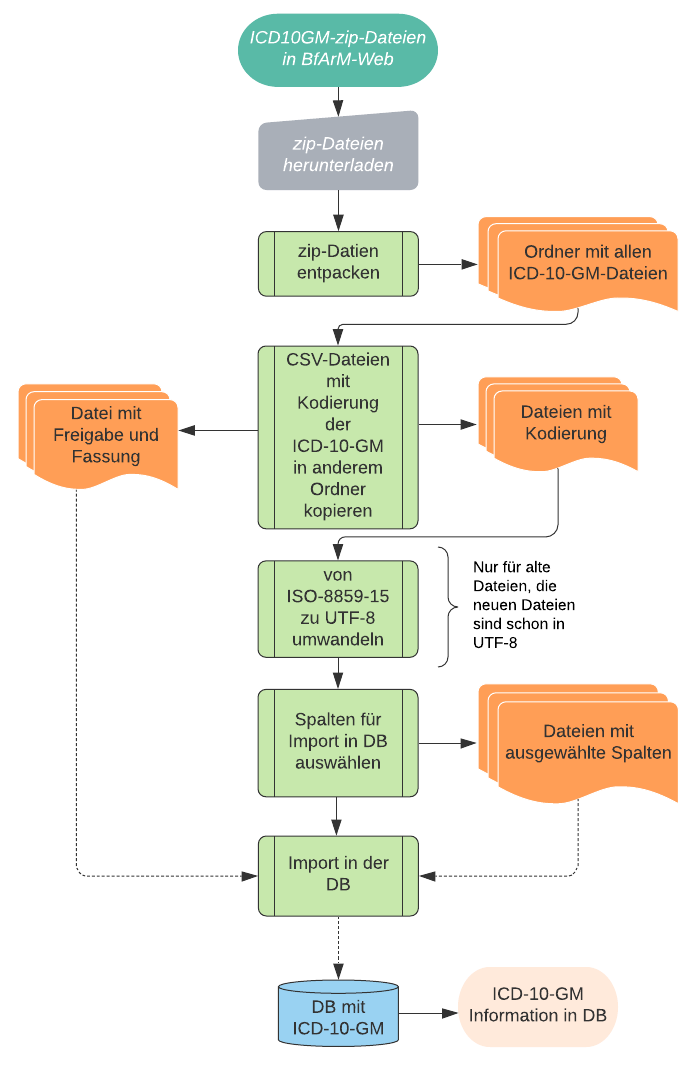
\includegraphics[height=14cm]{figures/etl}
		\caption[\acs{etl}-Strecke]{Flussdiagramm der \acs{etl}-Strecke für den Import der Information der \ac{icd10gm} von den \ac{zip}-Dateien in der \ac{db} }
		\label{fig:etl}
	\end{figure} 
	